\section{Event Detector Accuracy}
\label{evaluation-sec-eventdetection}

Our network was designed to capture interesting volcanic signals.  Thus, it
is critical that the system correctly identify and report such events.  This
section evaluates our event detection algorithm both in terms of the number
and rate of event triggers as well as its ability to detect scientifically
interesting events.

\subsection{Event triggers per node}

\begin{figure}[t]
\label{evaluation-fig-eventspernode}
\begin{center}
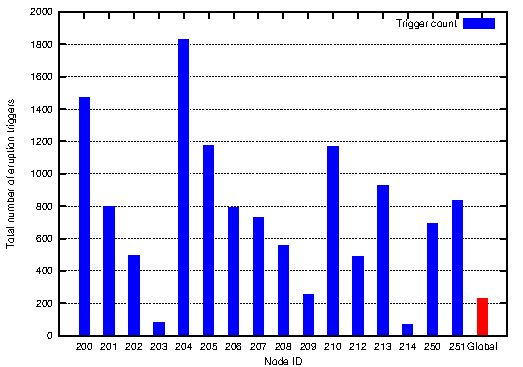
\includegraphics[width=\hsize]{./5-evaluation/figs/eventdetection/eruptionTriggers/eruptCount.pdf}
\end{center}
\caption{\textbf{Event triggers per node.}
This figure shows the total number of event triggers reported by each node.
It demonstrates a wide variation in trigger rates that cannot be attributed
only to varying node uptimes. For example, node~204 had the lowest uptime but
the largest number of event triggers.}
\end{figure}

\begin{figure}[t]
\label{evaluation-fig-eventspertime}
\begin{center}
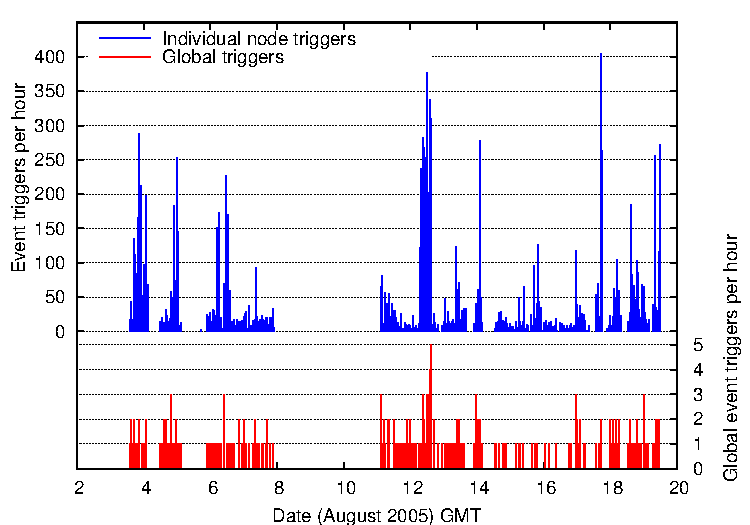
\includegraphics[width=\hsize]{./5-evaluation/figs/eventdetection/eruptionTriggers/eruptCountVsTime.pdf}
\end{center}
\caption{\textbf{Event triggers over time.}
The upper graph shows the total number of individual node triggers per hour.
The lower graph shows the corresponding number of global triggers.
Reventador's varying seismic activity generated between 0~to~5 global
triggers per hour.}
\end{figure}

Figure~\ref{evaluation-fig-eventspernode} shows the total number of events
reported by each node during the deployment. It shows a wide variation in the
event trigger rate, from 70~triggers for node~213 to 1830~triggers for
node~204.  Variation in the trigger rate can be attributed to many factors,
including the location of the node, the orientation of the seismometer, and
the quality of the seismometer-to-ground coupling.  Note that the trigger
rate does not seem to be related to distance from the vent. Although node~204
was closest to the vent and reported the most triggers, nodes 200, 205, and
210 all had high trigger counts despite being significantly farther away.

\subsection{Event triggers over time}

Figure~\ref{evaluation-fig-eventspertime} shows both the number of individual
node and global event triggers over each hour. We observe that the volcano's
activity varied greatly, generating trigger counts ranging between~2~and~405
events per hour when the network was online.  This activity translates into
up to 5~global event triggers an hour, each initiating a Fetch download cycle
of the associated data.

The volcano's bursty and unpredictable activity makes the network's design
more challenging than systems designed for statically-scheduled data
collection.  The data collection protocol, based on our earlier deployment at
Tungurahua~\cite{volcano-ewsn05}, assumed that events would be rare and that
it would be unnecessary to simultaneously record signals for one event while
downloading another. As a result, we missed a number of impressive
back-to-back eruptions typical of the activity at Reventador. It is worth
noting that the variable number of event reports is itself a measure of the
volcano's activity level and could be used to assess hazard levels. 

\subsection{Event detector accuracy}
\label{sec-eventdetectaccuracy}

%  - Event detector accuracy vs. Reftek data [MDW]
%    - Vary E.D. parameters

The network detected 229~eruptions, explosions, earthquakes, and tremor
events during the deployment. Ideally, we would like to assess its accuracy
in terms of the fraction of true events detected, as well as the false
positive rate. Given the high degree of coherence required by the global
event detector (requiring 30\% of the active nodes to trigger within a short
time window), we would be surprised if the sensor network recorded any false
events. Indeed, all of the signals we did capture appear to be based on true
volcanic activity, indicating a zero false positive rate.

We intended to apply our event detection algorithm to the signals collected
by the two broadband seismic stations to establish the algorithm's accuracy.
Unfortunately, we found this to be difficult for several reasons.  First,
each of the broadband stations suffered intermittent power and software
failures, either preventing them from logging any data, or corrupting the
collected signals or timestamps.  Thus, even in those cases where broadband
data is available, it is not always accurate. 
%Moreover, intermittent noise on a single broadband station could be
%interpreted as an event by our algorithm, yielding an artificially high
%trigger rate. 
Second, the broadband stations deployed a more sensitive seismometer with a
much wider frequency response.  The geophones used by our sensor nodes have a
corner frequency of 4.5~Hz, while the broadband sensors have a corner
frequency of 0.033~Hz.  Additionally, the broadband seismometers are much
more sensitive, generating voltages of 800~V/m/sec, whereas the geophones
have a sensitivity of only 32~V/m/sec. As a result, the broadband sensors are
able to detect much weaker seismic signals.

We focus our attention on a single day of data where the broadband stations
were recording clean data and the sensor network was relatively stable. One
of the authors, a seismologist, visually extracted events from the broadband
data; during this 24-hour period, a total of 589~events were recorded by the
broadband sensors. During the same time, the sensor network triggered on just
7~events, suggesting that our detection accuracy is very low (about 1\%).

The network could have failed to detect a seismic event for one of four
reasons: (1) failure of individual nodes; (2) failure of the base station or
radio modem; (3) the low sensitivity of our seismometers; or (4) failure of
the event detection algorithm itself. To factor out the increased sensitivity
of the broadband seismometers, we only consider the 174~events with SNR~$\geq
10$ from both stations, which we expect the geophones should have been able
to detect as well.  Also, Section~\ref{evaluation-sec-robustness} has already
addressed the question of uptime, so we focus here on the inherent accuracy
of the event detector when the network was operating correctly. 136~of the
174~broadband events occurred during times when the network was operational.
Taking these two factors into account, the network's detection accuracy is
still only about 5\%. 

%It is not
%clear how to tune the event detection algorithm for the broadband data.
%If the algorithm is not sensitive enough, it will fail to detect events that
%our network did in fact report.  If the algorithm is too sensitive, it will
%report false events that the sensor network should not have reported. 
%Although our EWMA-based algorithm was developed after consultation
%with seismologists, there is no single gold standard for event detection in
%the volcanological community.
%However, we did not experiment with different event-detection parameters in
%the field, as the number of eruptions and earthquakes triggering the current
%detector was more than adequate to exercise the network.  For our deployment
%the sheer volume of data precludes manual selection of events.

%In an attempt to assess the event detector's accuracy, we
%applied our original event-detection algorithm to the filtered 
%broadband data from August~11--19, which corresponds to 143~events 
%captured by our sensor network. 75~out of these~143 events (52\%) 
%have a trigger from at least one broadband station; 47~events (32\%)
%have triggers from both stations. The lack of triggers for the 
%remaining events (all of which are true seismic activity) 
%is due to corruption or gaps in the broadband data. 

%143~events from August 11--19 which were properly time rectified as described
%in Section~\ref{sec-timing}.  Of these events, 142 had corresponding data
%from at least one broadband station.  We then ran the original event
%detection algorithm on the broadband signals.
%%In addition, we lowered the EWMA ratio threshold of the detector from 1050
%%to 1030, making the detector much more sensitive than the mote detector.
%Due to the small number of broadband stations we consider a trigger from 
%{\em either} station as identifying a meaningful event. This implies that
%noise on a single station can increase our false positive rate.

% PARAMETERS USED HERE:
%   - Broadband event detector: low gain 1.0, high gain 9.0, threshold 1050
%   - Vote count required: 1 
%   - No suppression
%This resulted in 12505~individual triggers from the broadband data.
%123~out of the~142~events (87\%) had a
%corresponding trigger in the broadband data.  
%Given the high degree of
%coherence required by the global event detector (requiring 5~nodes to
%trigger within a short time window), we would be surprised if the sensor
%network recorded any spurious events. Indeed, all of the signals we did
%capture appear to be based on true volcanic activity.  
%We suspect that the
%lack of triggers for the remaining 19~events is due to corruption in the
%broadband data.
%However, with only 3~broadband stations, any one of
%which could have been faulty at any time, it is difficult to use this
%data to definitively evaluate event detection accuracy. 

%%%%%%%%%%%%%%%%%%%%%%%%%%%%%%%%%%%%%%%%%%%%%%%%%%%%%%%%%%%%%%%%%%%%%%%%%%%%
%%% MDW: Original text here:
%The more difficult question is what fraction of ``true'' events were
%successfully detected. As discussed above, without a gold standard for event
%detection and complete broadband data coverage, it is impossible to make 
%a direct comparison. The best we can do is use our original 
%event-detection algorithm on the broadband data and compare the 
%set of triggers to those reported by our network.
%
%Using the same global detector parameters (requiring both broadband
%stations to trigger within a 10~sec window) 
%yields 285 events in the broadband data set.
%%(a significant reduction from the 12505 individual triggers, suggesting very
%%high noise in the broadband data).
%Of these, 36 events (13\%) correspond to events recorded by our network.
%Each of remaining 249 missing events is the result of either the failure of
%the event detector, the failure of the sensor network, or false positives
%in the broadband data set. With only two broadband stations it is
%difficult to tease these reasons apart.  Of the 136 broadband events that
%occurred while all 16~nodes of the sensor network were operational, our
%network detected~24. If the broadband stations are considered ground truth
%this results in a detection accuracy of 17.7\%. 
%%%%%%%%%%%%%%%%%%%%%%%%%%%%%%%%%%%%%%%%%%%%%%%%%%%%%%%%%%%%%%%%%%%%%%%%%%%%

%%%%%%%%%%%%%%%%%%%%%%%%%%%%%%%%%%%%%%%%%%%%%%%%%%%%%%%%%%%%%%%%%%%%%%%%%%%%
%%% MDW: New text here:

%Without complete broadband data coverage, there is no way to tell how
%many true events occurred.  For sake of argument, let us consider the set
%of seismic events triggered in {\em both} broadband stations, a total
%of 406~triggers, as ``ground truth.''  However, because there are only
%two broadband stations, we expect a high false positive rate in the
%broadband data.  For example, if we had required only two~sensor votes 
%to trigger (rather than five), the number of sensor node events jumps 
%from 70~to~462 (an increase of 660\%) suggesting that the broadband
%trigger rate is artificially high.

%To compare the sensor network and broadband triggers, 
%We dilate each broadband trigger by 60~sec and consider
%any sensor network trigger that falls within this window to be 
%a match. 27~out of~the~70~(38\%) sensor network triggers match some 
%broadband trigger. Combining the broadband and sensor network
%triggers, there are 449~unique events; the sensor network detected 6\%. 
%However, it is worth noting
%that the broadband station missed 43~of the 70~sensor network events,
%likely due to missing data. The fact that the
%sensor network and broadband triggers are poorly correlated
%suggests that using the broadband stations is not an accurate 
%measure of ground truth. 

Recall that during a Fetch download cycle, nodes disabled sampling to avoid
overwriting data in flash. Download cycles could take up to several minutes
{\em per node} (see Section~\ref{evaluation-sec-performance}), meaning that
there are significant time windows when the network was unable to detect new
events.  During the Fetch cycles on August 15, the broadband stations
recorded 42~events, 24\% of the total events detected.  This indicates that,
all else being equal, the sensor network could have detected approximately
24\% more events had we designed the protocol to sample and download
simultaneously. We plan to add this feature in the next version of our
system.

In the end, we believe that our low detection rate is the result of the
parameters used in the EWMA-based event detection algorithm.  These
parameters were chosen prior to the deployment, based on our experience with
detecting infrasonic events at a different volcano~\cite{volcano-ewsn05}. We
did not experiment with modifying them in the field. Indeed, using our
algorithm with these same parameters on the broadband data for August~15
detects only 101~events, a fraction of the events chosen manually by an
expert.  We plan to tune our event-detection parameters for future
deployments based on the data collected by the broadband stations.

%Because we cannot define ground truth in absolute terms, we cannot
%directly report on the specificity and sensitivity of our event detection
%algorithm. Instead, we verify that for each event recorded by the
%sensor network, the same event-detection algorithm applied to the
%corresponding broadband station data would have also reported an 
%event. This is a measure of how many ``false positives'' are reported
%by the sensor network but does not capture ``false negatives.''
%
%We took a representative set of 78~events that appear to have accurate 
%timing (as described in Section~\ref{sec-timing}). We then applied our
%original event-detection algorithm on the corresponding data from 
%the RRVEN and RHOTEL stations (eliding station RLAV3 for the reasons 
%described above). The same event-detection parameters were used as
%by the motes in the original deployment. As expected, the algorithm 
%applied to the broadband data triggered events in 100\% of these cases, 
%meaning that there are no false positive events in our data set.

%less consensus about what constitutes a ``real event.''
%It is an open question what proportion of ``true'' events we
%successfully captured. 

%Applying our
%original algorithm to the broadband data set for August 11--19 
%reports 315~unique events. During the same period the sensor network
%reported 144~events. Only 33 events, or 23\% of the events reported
%by the network, match in both data sets. This is due to many factors.

%\begin{figure*}[t]
%\begin{tabular}{|llllll|} \hline
%{\bf Suppression window} & 
%{\bf Broadband events} &
%{\bf Mote events} &
%{\bf Matching events} & 
%{\bf ``False positive'' \%} & 
%{\bf ``False negative'' \%} \\ \hline
%{\bf 1 votes needed, thresh 1050} & & & & & \\ \hline
% {\em none}	& 8031 & 144 & 89 & 38\% & 99\% \\  \hline
%{\bf 2 votes needed, thresh 1050} & & & & & \\ \hline
% {\em none}	& 3530 & 144 & 37 & 74\% & 99\% \\  \hline
%\end{tabular}
%\caption{\small \XXXnote{finish this!}}
%\end{figure*}
%
%  - Global detector accuracy [MDW]
%    - How well did global detector filter out false events
%    - Specificity/sensitivity analysis [MDW - hold off]


